\documentclass[a4paper]{article}

\usepackage[portuguese]{babel}
\usepackage{comment}
\usepackage[T1]{fontenc}
\usepackage[utf8]{inputenc}
\usepackage{hyperref}
\usepackage{graphicx}
\usepackage{float}
\usepackage{multirow}
\usepackage{indentfirst}
\usepackage{listings}
\usepackage[hypcap]{caption} % makes \ref point to top of figures and tables
\newcommand{\tab}[1]{\hspace{.2\textwidth}\rlap{#1}}

\begin{document}
\lstset{language=Pascal}
\begin{titlepage}

	\begin{center}

		
\includegraphics[width=6cm]{./title}\\[3cm]

		\textsc{\LARGE Sistemas de Informação e Bases de Dados}\\[1.5cm]

		\textsc{\Large 1ª Parte do Projeto}\\[1.5cm]


		


		\noindent
		\begin{minipage}{0.4\textwidth}
			\begin{flushleft} \large
				Diogo Proença, 75313
			\end{flushleft}
		\end{minipage}
		\begin{minipage}{0.4\textwidth}
			\begin{flushright} \large
				Diogo Martins, 75462
			\end{flushright}
		\end{minipage}
		
		\begin{minipage}{0.4\textwidth}
			\begin{flushright} \large
				Bernardo Gomes, 75573	
			\end{flushright}
		\end{minipage}

		\vfill

		{\large \today}


	\end{center}

\end{titlepage}
\hypersetup{%
    pdfborder = {0 0 0}
}

\tableofcontents
\pagenumbering{gobble}
\pagebreak

\pagenumbering{arabic}
\section{Criação das tabelas da base de dados}
Para a criação das tabelas na base de dados, as intruções de SQL utilizadas foram as seguintes:

\lstinputlisting{database.sql}

Relativamente às escolhas das variáveis o seguinte conjunto merece especial destaque:
\begin{itemize}

  \item \textbf{variável \textit{number} da tabela \textit{Patient}} $\rightarrow$ ao termos levado a cabo pesquisa relativa a \textit{Social Security Numbers} (SSN's) válidos, verificámos que este conjunto de números pode conter caracteres não numéricos ("-"). Além deste facto, pode também começar pelo número "0", o que invalida o uso de variáveis \textit{integer}, \textit{numeric} e \textit{decimal} caso contrário o número armazenado iria perder dígitos. Utiliza-se assim, a variável \textit{varchar};
  
  \item \textbf{variável \textit{phone} da tabela \textit{PAN}} $\rightarrow$ tendo em conta a existência de números de telefone com prefixo diferente em cada país (\textit{e.g.} Portugal - +351), e não sendo necessário que o paciente tenha um número do país onde o \textit{Medical Center} está localizado, utiliza-se a variável \textit{varchar};
  
  \item \textbf{variável \textit{serialnum} da tabela \textit{Device}} $\rightarrow$ utiliza-se a variável \textit{integer}. No entanto, poder-se-ia considerar também do tipo \textit{varchar} pelo facto de em alguns casos os números de série conterem caracteres. No entanto, não tendo sendo especificado nada no enunciado, e não tendo obtido nenhuma informação sobre os números de série de aparelhos médicos, considera-se o caso em que estes podem ser representados por um número;
  
  \item Para as tabelas \textit{Sensor} e \textit{Actuator} é utilizado o mesmo critério que a tabela anterior;
  
  \item \textbf{variável \textit{nut4code} da tabela \textit{Municipality}} $\rightarrow$ para esta tabela, considera-se apenas os códigos postais semelhantes a Portugal, identificados por quatro números, tal como o nome da variável indica;
  
  \item \textbf{variáveis \textit{start} e \textit{end} da tabela \textit{Period}} $\rightarrow$ escolhe-se o tipo \textit{date} pelo facto de as relações com esta entidade não necessitar de precisões ao nível HH:mm:ss;
  
  \item para as tabelas \textit{Period}, \textit{Wears}, \textit{Lives} e \textit{Connects} foi colocada uma verificação das datas \textit{check(start<=end)} de forma a garantir que o período está consistente;

  \item \textbf{variável \textit{datetime} das tabelas \textit{Reading} e \textit{Setting}} $\rightarrow$ escolhe-se o tipo \textit{timestamp} pelo facto de as medições médicas necessitarem de precisões ao nível HH:mm:ss;
  
  \item \textbf{variável \textit{value} das tabelas \textit{Reading} e \textit{Setting}} $\rightarrow$ escolhe-se o tipo \textit{numeric} pelo facto de permitir precisão ao nível de casas decimais.  
\end{itemize}
\pagebreak
Inicialmente, acrescentam-se as seguintes instruções de forma a apagar eventuais tabelas com o mesmo nome antes da criação das novas:

\lstinputlisting{drop.sql}

\section{\textit{Triggers} para prevenção de \textit{overlapping periods}}
A função dos \textit{triggers} é de prevenir a inserção de associações a PAN's por parte de pacientes ou de aparelhos médicos em periodos de tempo sobrepostos. 

A \textit{error message} deve ser apresentada de forma a evitar que ocorram casos,  para a tabela \textit{Wears}, como os seguintes:
\vskip 5mm
\begin{itemize}
\item Paciente 1 está ligado a PAN1 e PAN2 ao mesmo tempo;

\item  Paciente 1 e Paciente 2 estão ligados à PAN1 ao mesmo tempo.
\end{itemize}

A \textit{error message} deve ser apresentada de forma a evitar que ocorram casos,  para a tabela \textit{Connects}, como o seguinte: 

\begin{itemize}

\item Device 1 está ligado a PAN1 e PAN2 ao mesmo tempo.

\end{itemize}
\pagebreak
\subsection{\textit{Triggers} de \textit{insert}}

Os triggers desenvolvidos foram os seguintes:

\lstinputlisting{insert.sql}

Por forma a testar o funcionamento dos \textit{triggers} atrás apresentados, utilizámos a base de dados fornecida no ficheiro \textit{database\_triggers\_insert.sql}. Após correr as instruções, obtêm-se as seguintes tabelas:
\begin{figure}[ht!]
\centering
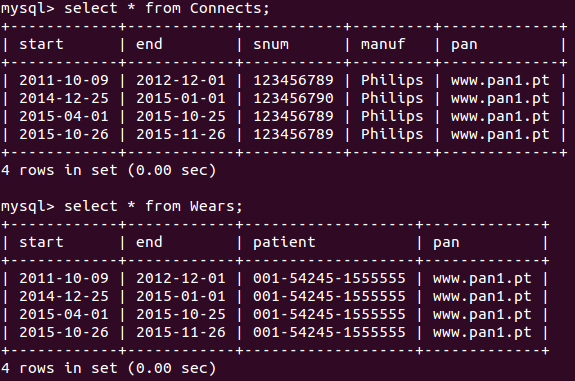
\includegraphics[scale=0.7]{tabelas_insert_triggers.png}
\caption{Tabelas para teste de \textit{insert} dos \textit{triggers}}
\end{figure}

Os testes realizados foram sucessivas inserções de um dispositivo em PAN's diferentes sobreposto a pelo menos uma entrada da tabela.

Os testes realizados estão contidos no ficheiro \textit{•}

\subsection{\textit{Triggers} de \textit{insert}}

\end{document}